

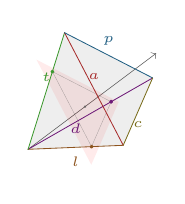
\begin{tikzpicture}[line join = round, line cap = round]

\coordinate (A) at (0.8737734,0.4020789,0.2735919); % incident to DPC (event node)
\coordinate (B) at (-0.5404401,0.6813372,-0.493664); % incident to TPA (step clocks!)
\coordinate (C) at (0.1666667,-0.787218,-0.5937256); % incident to LAC (origin anchor)
\coordinate (D) at (-0.5,-0.2961981,0.8137977); % incident to TLD (destination anchor)


% median lines: pick one
% \draw[->,color={rgb:red,1;green,1;blue,1}, densely dotted, line width = {0.2pt}] (A) -- (3*-0.2912578, 3*-0.1340263, 3*-0.0911973); % $TAL$ median
% \draw[->,color={rgb:red,1;green,1;blue,1}, densely dotted, line width = {0.2pt}] (B) -- (3*0.1801467, 3*-0.2271124, 3*0.1645547); % CDL median
% \draw[->,color={rgb:red,1;green,1;blue,1}, densely dotted, line width = {0.2pt}] (C) -- (3*-0.0555556, 3*0.262406, 3*0.1979085); % TPD median;
\draw[->,color={rgb:red,1;green,1;blue,1}, line width = {0.2pt}] (D) -- (3*0.1666667, 3*0.0987327, 3*-0.2712659); % APC median;

% bimedian lines: pick one
% \draw[->,color={rgb:red,1;green,1;blue,1}, densely dotted, line width = {0.2pt}] (1.3*-0.16666665,1.3*-0.54170805,1.3*0.11003605) -- (1.3*0.16666665,1.3*0.54170805,1.3*-0.11003605); % $LP$ bimedian
% \draw[->,color={rgb:red,1;green,1;blue,1}, densely dotted, line width = {0.2pt}] (1.3*-0.1868867,1.3*-0.0529404,1.3*-0.5436948) -- (1.1*0.1868867,1.3*0.0529404,1.3*0.5436948); % $AD$ bimedian
% \draw[->,color={rgb:red,1;green,1;blue,1}, densely dotted, line width = {0.2pt}] (1.3*-0.52022005,1.3*0.19256955,1.3*0.16006685) -- (1.3*0.52022005,1.3*-0.19256955,1.3*-0.16006685); % $TC$ bimedian

% redish transparent independent plane passing through midpoint 
% (match to bimedian line)
% bimed plane
%\fill[-, fill={rgb:red,1;green,0;blue,0}, opacity=.08] (0.7283081,-0.2695973,-0.2240936)--(0.2616414,0.0741166,0.7611727)--(-0.7283081,0.2695973,0.2240936)--(-0.2616414,-0.0741166,-0.7611727)--cycle; 

 % bimed intersection plane
%\draw[-, color={rgb:red,1;green,1;blue,1}, opacity=.5, line width = {0.1pt}] (0.5202201,-0.1925695,-0.1600669)--(0.1868867,0.0529404,0.5436948)--(-0.5202201,0.1925695,0.1600669)--(-0.1868867,-0.0529404,-0.5436948)--cycle;
% 0,0,0
%\node[mark size=.3pt,color={rgb:red,1;green,1;blue,1}, opacity=.5] at (0,0,0) {\pgfuseplotmark{*}}; 


% redish transparent triad plane passing through midpoint 
% (match to median line)
% med plane
\fill[-, fill={rgb:red,1;green,0;blue,0}, opacity=.08] (0.5821886,0.2370479,0.6351246)--(-0.7377441,0.4976889,-0.0809808)--(-0.0777778,-0.8729626,-0.1743716)--cycle; 

 % med intersection plane
\draw[-, color={rgb:red,1;green,1;blue,1}, opacity=.5, line width = {0.1pt}] (0.415849,0.1693199,0.4536605)--(-0.5269601,0.3554921,-0.0578434)--(-0.0555556,-0.6235447,-0.1245512)--cycle;
% tri centroid:
\node[mark size=.3pt,color={rgb:red,1;green,1;blue,1}, opacity=.5] at (-0.05555556,-0.0329109,0.09042196) {\pgfuseplotmark{*}}; 





% light shaded faces
\fill[-, fill={rgb:red,1;green,1;blue,1}, opacity=.05] (A)--(D)--(B)--cycle;       % TDP
\fill[-, fill={rgb:red,1;green,1;blue,1}, opacity=.05] (A)--(D)--(C)--cycle;       % CDL
\fill[-, fill={rgb:red,1;green,1;blue,1}, opacity=.05] (B)--(D)--(C)--cycle;       % TAL
\fill[-, fill={rgb:red,1;green,1;blue,1}, opacity=.05] (A)--(B)--(C)--cycle;       % APC

% color edges
\draw[-, color ={rgb:red,136;green,31;blue,147}, line width = {0.3pt}] (A)--(D);   % D
\draw[-, color ={rgb:red,197;green,117;blue,43}, line width = {0.3pt}] (D)--(C);   % L
\draw[-, color ={rgb:red,78;green,201;blue,59}, line width = {0.3pt}] (D)--(B);    % T
\draw[-, color ={rgb:red,210;green,55;blue,55}, line width = {0.3pt}] (B)--(C);    % A
\draw[-, color ={rgb:red,49;green,145;blue,201}, line width = {0.3pt}] (A)--(B);   % P
\draw[-, color ={rgb:red,210;green,188;blue,45}, line width = {0.3pt}] (A)--(C);   % C

% edge labels
% temp positions: above;below;below left; above; below
\node[above, color={rgb:red,49;green,145;blue,201}] at (0.16666665,0.54170805,-0.11003605) {\tiny $p$};      % AB mean
\node[below, color={rgb:red,210;green,188;blue,45}] at (0.52022005,-0.19256955,-0.16006685) {\tiny$c$};       % AC mean
\node[below left, color={rgb:red,136;green,31;blue,147}] at (0.1868867,0.0529404,0.5436948) {\tiny$d$};  % AD mean
\node[above, color={rgb:red,78;green,201;blue,59}] at (-0.52022005,0.19256955,0.16006685) {\tiny$t$};        % BD mean
\node[below, color={rgb:red,197;green,117;blue,43}] at (-0.16666665,-0.54170805,0.11003605) {\tiny$l$};       % CD mean
\node[above, color={rgb:red,210;green,55;blue,55}] at (-0.1868867,-0.0529404,-0.5436948) {\tiny$a$};        % BC mean

% bimedian line intersection points:
% P midpoint
%\node[mark size=.5pt,color={rgb:red,49;green,145;blue,201}] at (0.16666665,0.54170805,-0.11003605) {\pgfuseplotmark{*}}; 
% C midpoint
%\node[mark size=.5pt,color={rgb:red,210;green,188;blue,45}] at (0.52022005,-0.19256955,-0.16006685) {\pgfuseplotmark{*}}; 
 % D midpoint
%\node[mark size=.5pt,color={rgb:red,136;green,31;blue,147}] at (0.1868867,0.0529404,0.5436948) {\pgfuseplotmark{*}}; 
% T midpoint
%\node[mark size=.5pt,color={rgb:red,78;green,201;blue,59}] at (-0.52022005,0.19256955,0.16006685) {\pgfuseplotmark{*}}; 
% L midpoint
%\node[mark size=.5pt,color={rgb:red,197;green,117;blue,43}] at (-0.16666665,-0.54170805,0.11003605) {\pgfuseplotmark{*}}; 
% A midpoint
%\node[mark size=.5pt,color={rgb:red,210;green,55;blue,55}] at (-0.1868867,-0.0529404,-0.5436948) {\pgfuseplotmark{*}}; 

% median plan intersection points
% intersection 1
\node[mark size=.5pt,color={rgb:red,136;green,31;blue,147}] at (0.415849,0.1693199,0.4536605) {\pgfuseplotmark{*}}; % d
%  2
\node[mark size=.5pt,color={rgb:red,78;green,201;blue,59}] at (-0.5269601,0.3554921,-0.0578434) {\pgfuseplotmark{*}}; % t
 % 3 (match color by checking about) 
\node[mark size=.5pt,color={rgb:red,197;green,117;blue,43}] at (-0.0555556,-0.6235447,-0.1245512) {\pgfuseplotmark{*}}; % l
% helper dots for getting colors right :-)
% \node at (0.415849,0.1693199,0.4536605) {\tiny $1$};      
% \node at (-0.5269601,0.3554921,-0.0578434) {\tiny$2$};       
% \node at (-0.5269601,0.3554921,-0.0578434) {\tiny$3$};  


% node helper labels
% \node at (A) {\small A};
% \node at (B) {\small B};
% \node at (C) {\small C};
% \node at (D) {\small D};

\end{tikzpicture}

